 Insight Maker is a powerful online tool used to model and simulate complex systems. It utilizes different approaches, such as System Dynamics, Agent-Based Modeling and imperative programming. Insight Maker permits  construction of a graphical model to forecast the system response \cite{FortmannRoe}. We used the InsightMaker platform to prototype our model and simulate stepping forward through time. More details about the platform and its functionality can be found in Fortmann-Roe's review \cite{FortmannRoe}. The platform uses a fourth order Runge-Kutta differential equation solver for the system dynamics model and  first order Euler approximation for the Agent-Based model.\\

\noindent A normalized population fraction was simulated. The compartment S was initialized with a value of 999.999/1.000.000, and the compartment I with 1/1.000.000, meaning that there is an infected individual per every million of individuals, the rest of the compartments were set to zero as an initial condition. The flow between the compartments is given in the equations and all the other parameters were initialized as shown in Table \ref{tab:parameters}.  As mention at the beggining of the section, the parameters were calibrated in two stages, before and after the international intervention. According with the time frame proposed, the change in the parameters was also implemented on Insight Maker. The links to the online models can be found on \cite{IM_AI} and  \cite{IM_BI}.  


% RESULTS AND DISCUSSION
%
%No intervention
\noindent After modeling the system with the parameters before the intervention, it can be observed in Figure \ref{fig:LB_IM_NoIn} how the total population decreases to 46.46\%  if there is no intervention and the each of the parameters continue to be the same. The number of susceptible individuals exponentially decays, converging to 7\% of the population, while exposed, infected, hospitalized and funeral comparments converges to zero; finally, after the system stabilizes, the final proportion of deaths would be 53.53\% 

\begin{figure}[!h]
  \centering
  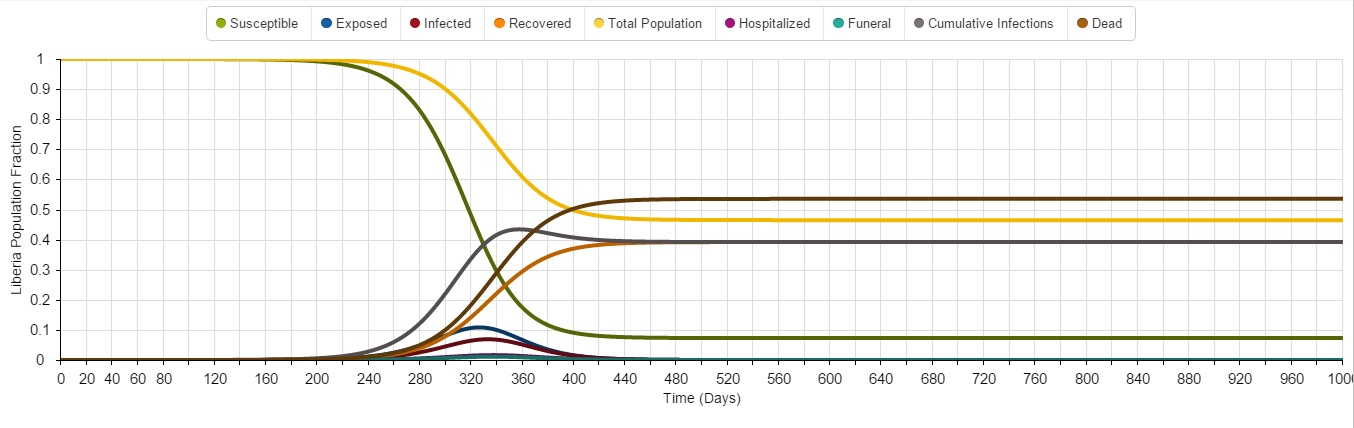
\includegraphics[width=1\textwidth]{LB_NoInt_SD_IM}
  \caption{ Insight Maker results using the parameters of the first stage (Mar/14 to Sept/14) and assuming no intervention}
\label{fig:LB_IM_NoIn} 
\end{figure}

%Intervention 
\noindent As mentioned before, five parameters were calibrated for the second stage of the Ebola Outbreak, namely, community contact rate ($\beta_I$), hospital contact rate ($\beta_H$), funeral contact rate ($\beta_F$), time until hospitalization ($\gamma_H$) and probability a case is hospitalized ($\theta$). Figure \ref{fig:LB_IM_In} A. shows that there is not much change in the Total population and susceptible compartment, meaning that the virus was controlled;  Figure \ref{fig:LB_IM_In} B focuses on E, I, R, H , F and D compartments, showing that the international intervention causes a dramatic change in the behavior of such compartments.

\begin{figure}[!h]
  \centering
  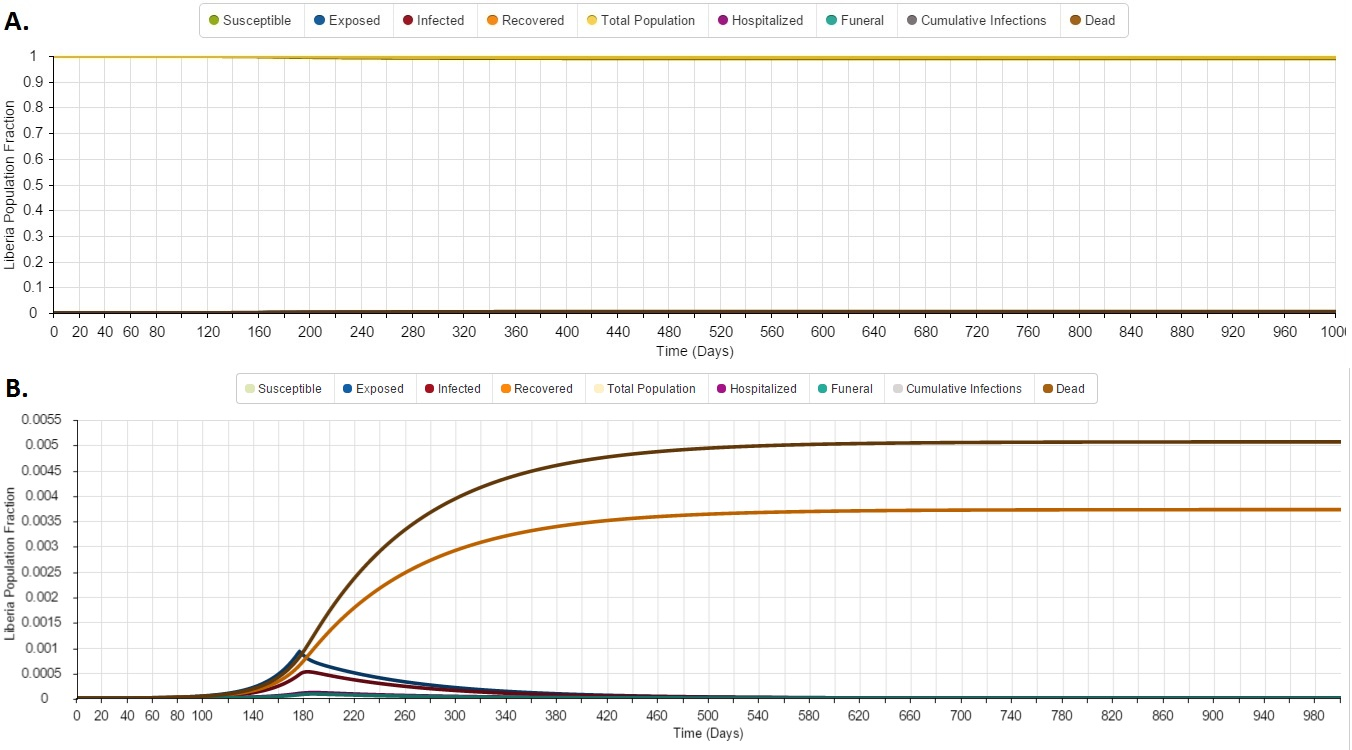
\includegraphics[width=1\textwidth]{LB_Int3_SD_IM}
  \caption{ Insight Maker results. \textit{A.} Parameters of the first stage (Mar/14 to Sept/14), \textit{B.} Parameters of the second stage ( Sept/14 to July/15)}
\label{fig:LB_IM_In} 
\end{figure}


%Comparing with WHO data

\noindent Finally, a comparison between the proposed model and World Health Organization data is shown in Figures \ref{fig:LB_IM_WHO} and \ref{fig:LB_IM_WHO2}. As depicted in Figure \ref{fig:LB_IM_WHO} A and B there is a good fitting of our model with the data reported by WHO. Figure \ref{fig:LB_IM_WHO2} shows  the reported WHO data before and after intervention, the results of our model before and after intervention and the forecast for the coming months, predicting that after the system reaches an equilibrium, the proportion of deaths in Liberia product of the EVD would be 5.07\% approximately.


\begin{figure}[!h]
  \centering
  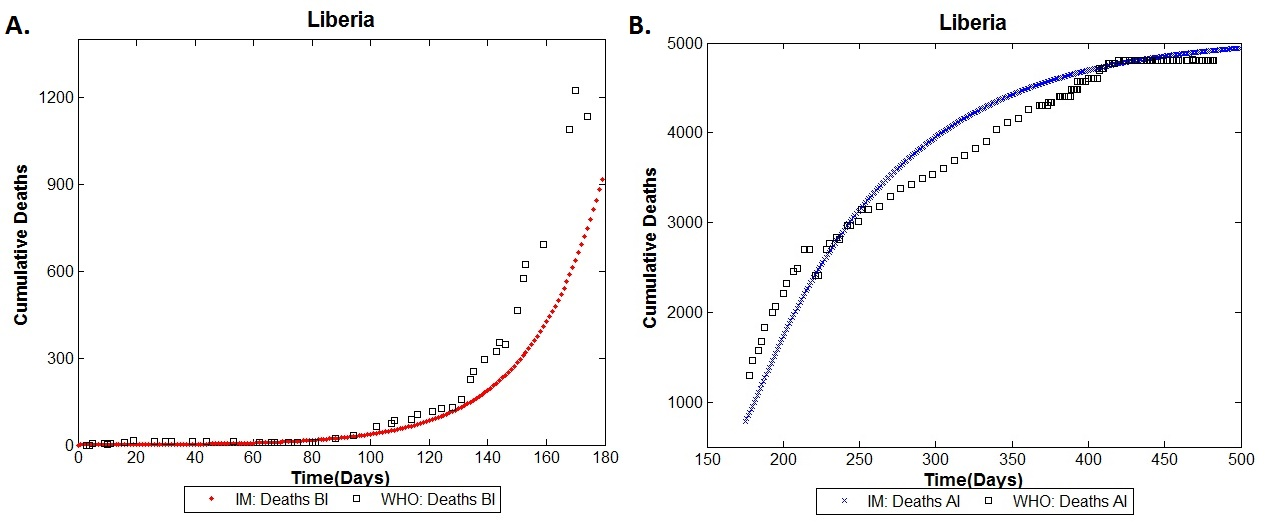
\includegraphics[width=1\textwidth]{LB_BI_AI_SD_WHO_IM}
  \caption{ Comparison between World Health Organization (WHO) data and Insight Maker (IM) results using the parameters of A. the first stage (Mar/14 to Sept/14) and B. the second stage ( Sept/14 to July/15) for the cumulative deaths (D).}
\label{fig:LB_IM_WHO} 
\end{figure}



\begin{figure}[!h]
  \centering
  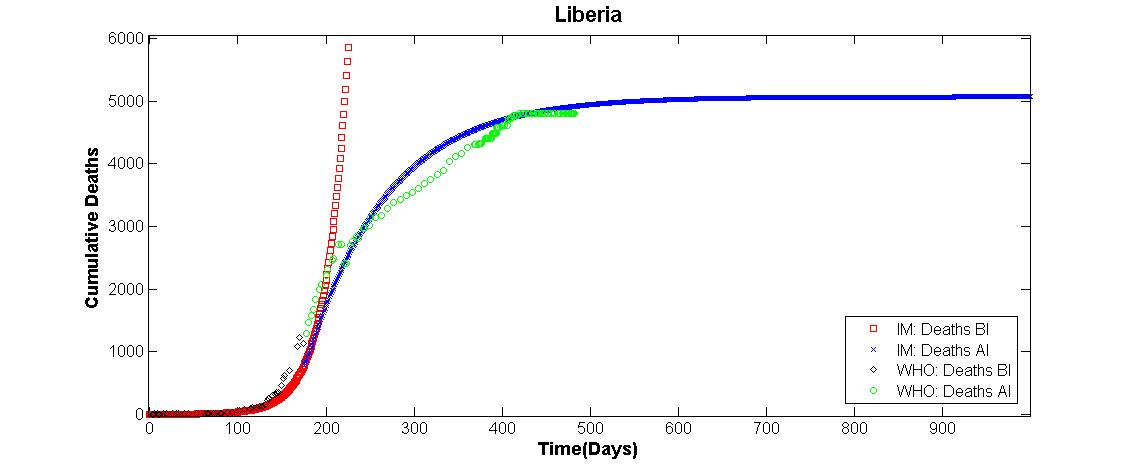
\includegraphics[width=1\textwidth]{LB_Int2_SD_WHO_IM}
  \caption{ Comparison between World Health Organization (WHO) data and Insight Maker (IM) results using the parameters before intervention (BI) and after intervention (AI), for the cumulative deaths (D).}
\label{fig:LB_IM_WHO2} 
\end{figure}


%%MATHEMATICA DESCRIPTION
Additionally, we drew the plots in the previous section also with Mathematica, and got almost same result. Furthermore, phase portraits of the system are shown in Figure \ref{fig:PhasePortrait}

\begin{figure}[!h]
  \centering
  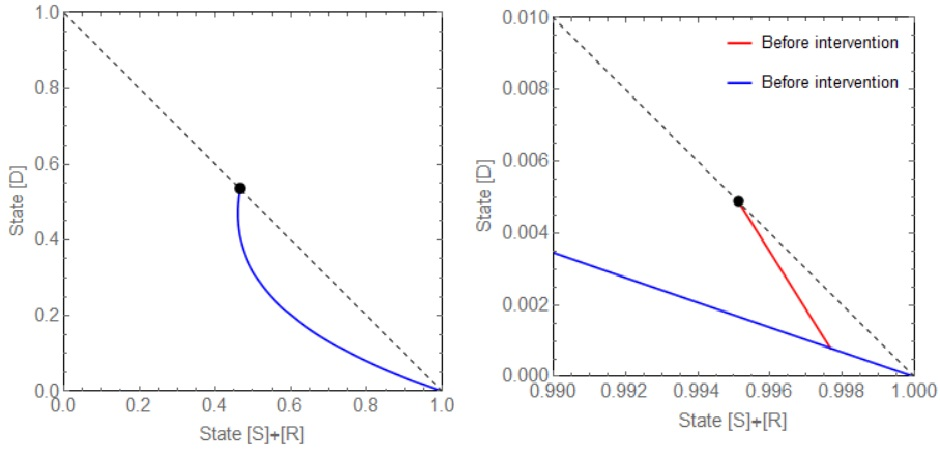
\includegraphics[width=1\textwidth]{PhasePortrait}
  \caption{Projection of phase portrait to (Susceptible + Recovered, Dead) space. (Blue) - without intervention, (Red) - with intervention, (Dots) - where the phase converges (equilibrium).}
\label{fig:PhasePortrait}
\end{figure}
